\documentclass[tikz,border=2mm]{standalone}
\usetikzlibrary{positioning,arrows.meta,calc,decorations.pathreplacing,shapes.geometric,fit}
\begin{document}
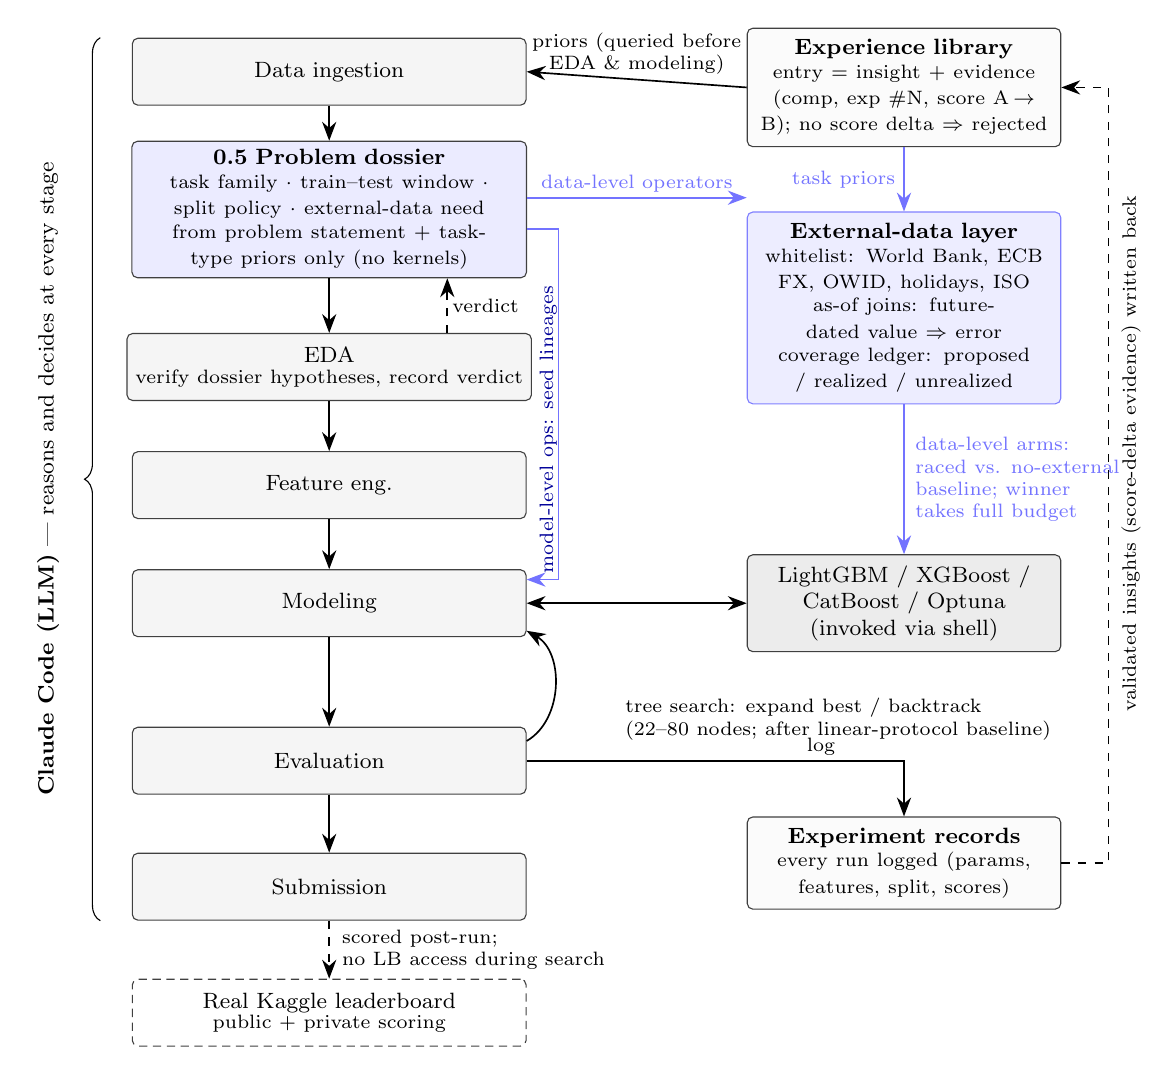
\begin{tikzpicture}[
  font=\footnotesize,
  stage/.style={draw=black!75, rounded corners=2pt, align=center, inner sep=3pt,
                fill=gray!8, minimum height=8.5mm, minimum width=50mm},
  supp/.style={draw=black!75, rounded corners=2pt, align=center, inner sep=4pt,
               fill=gray!3, text width=37mm},
  injbox/.style={supp, fill=blue!7, draw=blue!50},
  toolbox/.style={supp, fill=gray!15},
  arr/.style={-{Stealth[length=2.4mm]}, semithick},
  barr/.style={arr, blue!55},
  darr/.style={arr, dashed},
  lab/.style={font=\scriptsize, inner sep=1.5pt}
]
% ----- main pipeline (top -> bottom) -----
\node[stage]              (s1)  at (0,0)     {Data ingestion};
\node[stage, fill=blue!8, text width=48mm] (s05) at (0,-1.75)
  {\textbf{0.5 Problem dossier}\\[-1pt]
   {\scriptsize task family $\cdot$ train--test window $\cdot$ split policy $\cdot$ external-data need}\\[-1pt]
   {\scriptsize from problem statement + task-type priors only (no kernels)}};
\node[stage]              (s2)  at (0,-3.75)  {EDA\\[-2pt]{\scriptsize verify dossier hypotheses, record verdict}};
\node[stage]              (s3)  at (0,-5.25)  {Feature eng.};
\node[stage]              (s4)  at (0,-6.75)  {Modeling};
\node[stage]              (s5)  at (0,-8.75)  {Evaluation};
\node[stage]              (s6)  at (0,-10.35) {Submission};
\foreach \a/\b in {s1/s05, s05/s2, s2/s3, s3/s4, s4/s5, s5/s6}{\draw[arr] (\a) -- (\b);}
% ----- EDA verdict back to the dossier -----
\draw[darr] ([xshift=15mm]s2.north) -- node[lab, right]{verdict} ([xshift=15mm]s05.south);
% ----- pipeline endpoint: the real leaderboard -----
\node[stage, densely dashed, fill=white] (lb) at (0,-11.95)
  {Real Kaggle leaderboard\\[-2pt]{\scriptsize public + private scoring}};
\draw[darr] (s6) -- node[lab, anchor=west, xshift=1mm, align=left]
  {scored post-run;\\no LB access during search} (lb);
% ----- LLM annotation: vertical brace spanning all stages -----
\draw[decorate, decoration={brace, amplitude=2mm}]
  ([xshift=-4mm]s6.south west) -- ([xshift=-4mm]s1.north west)
  node[midway, xshift=-4mm, rotate=90, anchor=south]
  {\textbf{Claude Code (LLM)} --- reasons and decides at every stage};
% ----- tree-search loop (Evaluation -> Modeling), arc in the corridor -----
\draw[arr] ([yshift=2.5mm]s5.east) to[out=30, in=-30] ([yshift=-3.5mm]s4.east);
\node[lab, anchor=north west, align=left] at (3.7,-7.9)
  {tree search: expand best / backtrack\\(22--80 nodes; after linear-protocol baseline)};
% ----- right rail -----
\node[supp]    (lib)   at (7.3,-0.2)  {\textbf{Experience library}\\[-1pt]
  {\scriptsize entry = insight + evidence (comp, exp \#N, score A$\,\to\,$B); no score delta $\Rightarrow$ rejected}};
\node[injbox]  (ext)   at (7.3,-3.0)  {\textbf{External-data layer}\\[-1pt]
  {\scriptsize whitelist: World Bank, ECB FX, OWID, holidays, ISO}\\[-1pt]
  {\scriptsize as-of joins: future-dated value $\Rightarrow$ error}\\[-1pt]
  {\scriptsize coverage ledger: proposed / realized / unrealized}};
\node[toolbox] (tools) at (7.3,-6.75) {LightGBM / XGBoost /\\CatBoost / Optuna\\(invoked via shell)};
\node[supp]    (rec)   at (7.3,-10.05) {\textbf{Experiment records}\\[-1pt]
  {\scriptsize every run logged (params, features, split, scores)}};
% ----- rail / pipeline connections -----
\draw[arr]  (lib.west) -- node[lab, above, align=center]{priors (queried before\\EDA \& modeling)} (s1.east);
\draw[barr] (lib.south) -- node[lab, anchor=east, xshift=-0.5mm]{task priors} (ext.north);
\draw[barr] ([yshift=1.5mm]s05.east) -- node[lab, above]{data-level operators}
  ([yshift=1.5mm]ext.west |- s05.east);
% ----- model-level operators: dossier seeds the search directly -----
\draw[barr] ([yshift=-2.5mm]s05.east) -- ++(4mm,0) |- ([yshift=3mm]s4.east);
\node[lab, rotate=90, anchor=south, blue!60!black] at (2.95,-4.55)
  {model-level ops: seed lineages};
\draw[barr] (ext.south) -- node[lab, anchor=west, xshift=0.8mm, align=left]
  {data-level arms:\\raced vs. no-external\\baseline; winner\\takes full budget} (tools.north);
\draw[arr, {Stealth[length=2.4mm]}-{Stealth[length=2.4mm]}] (s4.east) -- (tools.west);
\draw[arr]  (s5.east) -- node[lab, above, pos=0.78]{log} (rec.north |- s5.east) -- (rec.north);
% ----- dashed write-back, up the far right -----
\draw[darr] (rec.east) -- ++(6mm,0) |- (lib.east);
\node[lab, rotate=90, anchor=north] at (10.0,-4.85)
  {validated insights (score-delta evidence) written back};
\end{tikzpicture}
\end{document}
